% THIS DOCUMENT IS TAILORED TO REQUIREMENTS FOR SCIENTIFIC COMPUTING.  IT SHOULDN'T
% BE USED FOR NON-SCIENTIFIC COMPUTING PROJECTS
\documentclass[12pt]{article}

\usepackage{amsmath, mathtools}
\usepackage{amsfonts}
\usepackage{amssymb}
\usepackage{graphicx}
\usepackage{colortbl}
\usepackage{xr}
\usepackage{hyperref}
\usepackage{longtable}
\usepackage{xfrac}
\usepackage{tabularx}
\usepackage{float}
\usepackage{siunitx}
\usepackage{booktabs}
\usepackage{caption}
\usepackage{pdflscape}
\usepackage{afterpage}


\usepackage[round]{natbib}

%\usepackage{refcheck}

\hypersetup{
    bookmarks=true,         % show bookmarks bar?
      colorlinks=true,       % false: boxed links; true: colored links
    linkcolor=red,          % color of internal links (change box color with linkbordercolor)
    citecolor=green,        % color of links to bibliography
    filecolor=magenta,      % color of file links
    urlcolor=cyan           % color of external links
}

%% Comments

\usepackage{color}

\newif\ifcomments\commentstrue %displays comments
%\newif\ifcomments\commentsfalse %so that comments do not display

\ifcomments
\newcommand{\authornote}[3]{\textcolor{#1}{[#3 ---#2]}}
\newcommand{\todo}[1]{\textcolor{red}{[TODO: #1]}}
\else
\newcommand{\authornote}[3]{}
\newcommand{\todo}[1]{}
\fi

\newcommand{\wss}[1]{\authornote{blue}{SS}{#1}} 
\newcommand{\plt}[1]{\authornote{magenta}{TPLT}{#1}} %For explanation of the template
\newcommand{\an}[1]{\authornote{cyan}{Author}{#1}}

%% Common Parts

\newcommand{\progname}{ProgName} % PUT YOUR PROGRAM NAME HERE
\newcommand{\authname}{Team \#, Team Name
\\ Student 1 name
\\ Student 2 name
\\ Student 3 name
\\ Student 4 name} % AUTHOR NAMES                  

\usepackage{hyperref}
    \hypersetup{colorlinks=true, linkcolor=blue, citecolor=blue, filecolor=blue,
                urlcolor=blue, unicode=false}
    \urlstyle{same}
                                


% For easy change of table widths
\newcommand{\colZwidth}{1.0\textwidth}
\newcommand{\colAwidth}{0.13\textwidth}
\newcommand{\colBwidth}{0.82\textwidth}
\newcommand{\colCwidth}{0.1\textwidth}
\newcommand{\colDwidth}{0.05\textwidth}
\newcommand{\colEwidth}{0.8\textwidth}
\newcommand{\colFwidth}{0.17\textwidth}
\newcommand{\colGwidth}{0.5\textwidth}
\newcommand{\colHwidth}{0.28\textwidth}

% Used so that cross-references have a meaningful prefix
\newcounter{defnum} %Definition Number
\newcommand{\dthedefnum}{GD\thedefnum}
\newcommand{\dref}[1]{GD\ref{#1}}
\newcounter{datadefnum} %Datadefinition Number
\newcommand{\ddthedatadefnum}{DD\thedatadefnum}
\newcommand{\ddref}[1]{DD\ref{#1}}
\newcounter{theorynum} %Theory Number
\newcommand{\tthetheorynum}{TM\thetheorynum}
\newcommand{\tref}[1]{TM\ref{#1}}
\newcounter{tablenum} %Table Number
\newcommand{\tbthetablenum}{TB\thetablenum}
\newcommand{\tbref}[1]{TB\ref{#1}}
\newcounter{assumpnum} %Assumption Number
\newcommand{\atheassumpnum}{A\theassumpnum}
\newcommand{\aref}[1]{A\ref{#1}}
\newcounter{goalnum} %Goal Number
\newcommand{\gthegoalnum}{GS\thegoalnum}
\newcommand{\gsref}[1]{GS\ref{#1}}
\newcounter{instnum} %Instance Number
\newcommand{\itheinstnum}{IM\theinstnum}
\newcommand{\iref}[1]{IM\ref{#1}}
\newcounter{reqnum} %Requirement Number
\newcommand{\rthereqnum}{R\thereqnum}
\newcommand{\rref}[1]{R\ref{#1}}
\newcounter{nfrnum} %NFR Number
\newcommand{\rthenfrnum}{NFR\thenfrnum}
\newcommand{\nfrref}[1]{NFR\ref{#1}}
\newcounter{lcnum} %Likely change number
\newcommand{\lthelcnum}{LC\thelcnum}
\newcommand{\lcref}[1]{LC\ref{#1}}

\usepackage{fullpage}

\newcommand{\deftheory}[9][Not Applicable]
{
\newpage
\noindent \rule{\textwidth}{0.5mm}

\paragraph{RefName: } \textbf{#2} \phantomsection 
\label{#2}

\paragraph{Label:} #3

\noindent \rule{\textwidth}{0.5mm}

\paragraph{Equation:}

#4

\paragraph{Description:}

#5

\paragraph{Notes:}

#6

\paragraph{Source:}

#7

\paragraph{Ref.\ By:}

#8

\paragraph{Preconditions for \hyperref[#2]{#2}:}
\label{#2_precond}

#9

\paragraph{Derivation for \hyperref[#2]{#2}:}
\label{#2_deriv}

#1

\noindent \rule{\textwidth}{0.5mm}

}

\begin{document}

\title{Software Requirements Specification for \progname: subtitle describing software} 
\author{\authname}
\date{\today}
	
\maketitle

~\newpage

\pagenumbering{roman}

\tableofcontents

~\newpage

\section*{Revision History}

\begin{tabularx}{\textwidth}{p{3cm}p{2cm}X}
\toprule {\bf Date} & {\bf Version} & {\bf Notes}\\
\midrule
Date 1 & 1.0 & Notes\\
Date 2 & 1.1 & Notes\\
\bottomrule
\end{tabularx}

\newpage

\pagenumbering{arabic}


\section{Introduction}

\plt{The introduction section is written to introduce the problem.  It starts
  general and focuses on the problem domain. The general advice is to start with
a paragraph or two that describes the problem, followed by a ``roadmap''
paragraph.  A roadmap orients the reader by telling them what sub-sections to
expect in the Introduction section.}

\subsection{Purpose of Document}

\plt{This section summarizes the purpose of the SRS document.  It does not focus
  on the problem itself.  The problem is described in the ``Problem
  Description'' section (Section~\ref{Sec_pd}).  The purpose is for the document
  in the context of the project itself, not in the context of this course.
  Although the ``purpose'' of the document is to get a grade, you should not
  mention this.  Instead, ``fake it'' as if this is a real project.  The purpose
  section will be similar between projects.  The purpose of the document is the
  purpose of the SRS, including communication, planning for the design stage,
  etc.}

\subsection{Characteristics of Intended Reader} \label{sec_IntendedReader}

\plt{This section summarizes the skills and knowledge of the readers of the
  SRS.  It does NOT have the same purpose as the ``User Characteristics''
  section (Section~\ref{SecUserCharacteristics}).  The intended readers are the
  people that will read, review and maintain the SRS.  They are the people that
  will conceivably design the software that is intended to meet the
  requirements.  The user, on the other hand, is the person that uses the
  software that is built.  They may never read this SRS document.  Of course,
  the same person could be a ``user'' and an ``intended reader.''}

\plt{The intended reader characteristics should be written as unambiguously and
  as specifically as possible.  Rather than say, the user should have an
  understanding of physics, say what kind of physics and at what level.  For
  instance, is high school physics adequate, or should the reader have had a
  graduate course on advanced quantum mechanics?}

\subsection{Scope of Requirements} 

\plt{Modelling the real world requires simplification.  The full complexity of
  the actual physics, chemistry, biology is too much for existing models, and
  for existing computational solution techniques.  Rather than say what is in
  the scope, it is usually easier to say what is not.  You can think of it as
  the scope is initially everything, and then it is constrained to create the
  actual scope.  For instance, the problem can be restricted to 2 dimensions, or
  it can ignore the effect of temperature (or pressure) on the material
  properties, etc.}  

\plt{The scope section is related to the assumptions section
  (Section~\ref{sec_assumpt}).  However, the scope and the assumptions are not
  at the same level of abstraction.  The scope is at a high level.  The focus is
  on the ``big picture'' assumptions.  The assumptions section lists, and
  describes, all of the assumptions.}

\plt{The scope section is relevant for later determining typical values of inputs. The scope should make it clear what inputs are reasonable to expect. This is a distinction between scope and context (context is a later section).  Scope affects the inputs while context affects how the software will be used.}

\plt{The goal statements refine the ``Problem Description''
  (Section~\ref{Sec_pd}).  A goal is a functional objective the system under
  consideration should achieve. Goals provide criteria for sufficient
  completeness of a requirements specification and for requirements
  pertinence. Goals will be refined in Section “Instanced Models”
  (Section~\ref{sec_instance}). Large and complex goals should be decomposed
  into smaller sub-goals.  The goals are written abstractly, with a minimal
  amount of technical language.  They should be understandable by non-domain
  experts.}

\noindent Given the \plt{inputs}, the goal statements are:

\begin{itemize}
\item[GS\refstepcounter{goalnum}\thegoalnum \label{G_meaningfulLabel}:] \plt{One
    sentence description of the goal.  There may be more than one.  Each Goal
    should have a meaningful label.}
\end{itemize}

% References at the end of the document

\subsection{Organization of Document}

\plt{This section provides a roadmap of the SRS document.  It will help the
  reader orient themselves.  It will provide direction that will help them
  select which sections they want to read, and in what order.  This section will
  be similar between project.}

~\newpage

\section{System Description}

\subsection{Definitions, Acronyms, and Abbreviations}

\plt{This section is expressed in words, not with equations.  It provide the
  meaning of the different words and phrases used in the domain of the problem.
The terminology is used to introduce concepts from the world outside of the
mathematical model  The terminology provides a real world connection to give the
mathematical model meaning.}

This subsection provides a list of terms that are used in the subsequent
sections and their meaning, with the purpose of reducing ambiguity and making it
easier to correctly understand the requirements:

\begin{itemize}
\item 
\end{itemize}

\subsection{System overview}

\subsection{System Functionality}

\subsection{User Characteristics} \label{SecUserCharacteristics}

\subsection{System Constraints}

\subsubsection{Assumptions and Dependencies} \label{sec_assumpt}
Here are some assumptions of the software--

\begin{itemize}
  \item\textbf{Software's Compatibility}--We are assuming that this voice recognition software will be compatible with the Health Record Database system of the hospitals. Moreover, we also assume that database system is accessible to keep the conversation secure and private in patient’s profile.
  \item\textbf{Patient's comfort}--We also assume that patient’s is comfortable using this software, ensuring that all sensitive information will be kept private.
  \item\textbf{Real-time Processing}--We assume that system is processing the conversation and filling the chart simultaneously, without any delay otherwise any delay in documentation will delete the purpose of this project.
  \item\textbf{Compatible with all templates}--Since hospitals and clinics have different templates for documenting a patient, we will assume AI is able to pick the key word of the question and fill it in.
\end{itemize}

Here are some dependencies of this software--

\begin{itemize}
  \item\textbf{Documentation template}-- Automation the documentation process depends on the type of template a doctor is using. For example, a dentist uses a different template compared to a medical doctor in emergency department.
  \item\textbf{Good sound input}-- The software depends on the type of input it is receiving from the doctor. A clear speech from the doctor and minimized background noise would provide more accurate results as compared to the noisy environment especially in emergency department.
  \item\textbf{Updating regularly}-- To function the system properly, it is required to update it on a regular basis, as any delay in updating the system would result in lost of information.
\end{itemize}


\subsubsection{Usage Scanerios}

Here are the use-case scenarios for this software--

\begin{itemize}
  \item\textbf{UC1 Document Consultation}--
  \begin{itemize}
    \item{Hospital staff logs into the system.}
    \item{Hospital staff will access patient’s profile.}
    \item{Dictation tool will be activated.}
    \item{Conversation between the doctor and the patient is captured.}
    \item{Audio is converted to text, automatically filling out the charts.}
  \end{itemize}
  \item\textbf{UC2 Generate Diagnosis Understandings}--
  \begin{itemize}
    \item{Software will analyze the patient’s symptoms from the recorded data.}
    \item{Based on the medical understanding, it will suggest some diagnoses methods.}
    \item{It will also assist the doctors by suggesting some treatment options.}
    \item{Medical doctor may accept or reject these suggestions, incorporating their professional judgement.}
  \end{itemize}
\end{itemize}

\textbf{Usage Scenario 1 : Documenting a Patient Consultation}

\begin{itemize}
  \item\textbf{Use Case}-- UC1,UC2
  \item\textbf{Primary Actor}-- Medical staff (such as a medical doctor or a nurse)
  \item\textbf{Precondition}-- Patient profile database system is accessible to the medical staff along with an electronic device (such as an iPad or a tablet)
  \item\textbf{Trigger}-- Medical professional wants to document patient’s condition and seek advice on diagnosis and treatment.
  \item\textbf{Main Success Scenario}--
  \begin{itemize}
    \item{The medical staff logs into the system and access the patient’s portfolio.}
    \item{The app presents the main dashboard with options to start a new documentation process for the patient.}
    \item{It will also show patient’s illness history and data from previous visit (if applicable).}
    \item{The voice recognition software is activated, and the medical staff starts the conversation with the patient.}
    \item{The audio data is then converted to text in real-time and the chart fields are automatically filled.}
    \item{Once the documentation is completed, the software starts suggesting diagnosis and other treatments options.}
  \end{itemize}
  \item\textbf{Secondary Success Scenario}--
  \begin{itemize}[label=1.\arabic*]
    \item{If the patient is visiting the doctor for the first time, a new profile is created.}
  \end{itemize}
  \begin{itemize}[label=4.\arabic*]
    \item{The doctor may use some external medical equipment such as BP measuring tool rather than speaking.}
  \end{itemize}
  \begin{itemize}[label=5.\arabic*]
    \item{The doctor may ask some private information (such as family’s illness history) and add it manually if it’s missing in the template.}
  \end{itemize}
  \begin{itemize}[label=6.\arabic*]
    \item{It's doctor’s decision to accept or reject software’s suggestions about the treatment and diagnosis options.}
  \end{itemize}
  \item\textbf{Success Postcondition}--
  \begin{itemize}
    \item{The medical staff will receive a summary of patient’s visit which will later be saved in their profile for privacy reasons.}
  \end{itemize}
\end{itemize}

\begin{figure}[h]
  \centering
  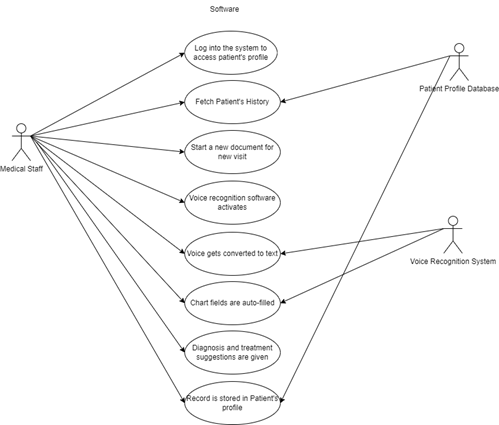
\includegraphics[width=0.8\textwidth]{use_case_diag.png}
  \caption{This is the use-case diagram for this project.}
  \label{fig:Use-Case Diagram}
\end{figure}

\begin{figure}[h]
  \centering
  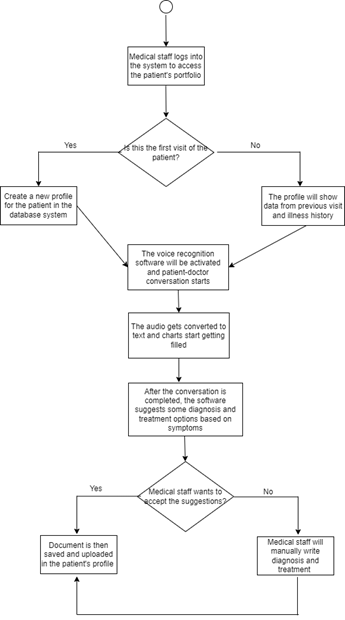
\includegraphics[width=0.8\textwidth]{activity_diag.png}
  \caption{This is the activity diagram for this project.}
  \label{fig:Activity Diagram}
\end{figure}

\subsubsection{Risks and Mitigation}

Looking at implementation details there are a few risks that come up, if these risks can be addressed or have a clearer roadmap that will make us more confident in the project. 

\begin{itemize}
  \item \textbf{Speech Input} -- A hospital or a clinic can be a loud place, in the event audio input is taken we need to ensure that it is clean and clear. This would mean essentially blocking outside noise. 
  \item \textbf{Visual Inputs} -- If any old charts need to be inputted into the patient journey having the ability to scan and transfer the information into the required format will be another risk. The document needs to be rid of noisy data.
  \item \textbf{Pre-Trained Models} -- To manipulate and use both inputs above we need to create a model to be accurate and provide accuracy when filling in charts. 
  \item \textbf{Data Privacy} -- This application will hold a lot of patient data so creating a store that is secure and making sure standard data security practice is applied is a must.
  \item \textbf{User Acceptance} -- This will require further elicitation from outside supervisors. We need to gather data on what critical needs of healthcare professionals such that critical features are present.
  \item \textbf{Technical Delay} – Integration with Electronic Health record systems might cause some delays if there’s any technical issue or if the software faces compatibility issues. This will require sample testing to make sure that the software is compatible in the early stage of the development process.
  \item \textbf{Professional Verification} – Misinterpretation of some words might lead to inaccurate records and wrong diagnosis. Therefore, it’s important for the doctor/nurse to verify the final version of the document and manually delete anything that was falsely recorded. 
\end{itemize}

~\newpage

\section{Requirements}

This section provides the functional requirements, the business tasks that the
software is expected to complete, and the nonfunctional requirements, the
qualities that the software is expected to exhibit.

\subsection{Functional Requirements}

\noindent \begin{itemize}

\item[R\refstepcounter{reqnum}\thereqnum \label{R_Inputs}:] \plt{Requirements
    for the inputs that are supplied by the user.  This information has to be
    explicit.}

\item[R\refstepcounter{reqnum}\thereqnum \label{R_OutputInputs}:] \plt{It isn't
    always required, but often echoing the inputs as part of the output is a
    good idea.}

\item[R\refstepcounter{reqnum}\thereqnum \label{R_Calculate}:] \plt{Calculation
    related requirements.}

\item[R\refstepcounter{reqnum}\thereqnum \label{R_VerifyOutput}:]
  \plt{Verification related requirements.}

\item[R\refstepcounter{reqnum}\thereqnum \label{R_Output}:] \plt{Output related
    requirements.}

\end{itemize}

\plt{Every IM should map to at least one requirement, but not every requirement
  has to map to a corresponding IM.}

\subsection{Non-functional Requirements}

\noindent \begin{itemize}

\item[NFR\refstepcounter{nfrnum}\thenfrnum \label{NFR_Performance}:] \textbf{Performance}  
    
    \textbf{Requirement:} The system shall process voice recordings and convert them into medical charts within 30 seconds of recording completion.  
  
    \textbf{Rationale:} Quick documentation is critical to streamline the patient journey and reduce healthcare professionals' workload.  
  
    \textbf{Fit Criterion:} The system will consistently generate completed documentation in under 30 seconds.  
  
    \textbf{Dependencies:} Dependent on the speech-to-text engine and cloud infrastructure.  
  
    \textbf{Normal Operation:} Under typical conditions, the system will handle up to 100 voice recordings per hour without performance degradation.  
  
    \textbf{Undesired Event Handling:} If the system takes longer than 30 seconds, an alert will be triggered, and the system will attempt to resolve delays by reducing background processes or scaling resources.

\item[NFR\refstepcounter{nfrnum}\thenfrnum \label{NFR_Reliability}:] \textbf{Reliability}  

    \textbf{Requirement:} The system shall have a 99.9\% uptime guarantee during operational hours (9 AM to 9 PM).  
  
    \textbf{Rationale:} Reliability is critical to ensure uninterrupted service for healthcare professionals, particularly in time-sensitive environments like emergency rooms.  
  
    \textbf{Fit Criterion:} System logs will confirm an uptime rate of 99.9\% over a 30-day period.  
  
    \textbf{Dependencies:} Cloud infrastructure, hosting services, and local hardware resilience.  
  
    \textbf{Undesired Event Handling:} If uptime falls below 99.9\%, an automated system will switch to backup servers within 10 seconds to ensure continuity of service.

\item[NFR\refstepcounter{nfrnum}\thenfrnum \label{NFR_Scalability}:] \textbf{Scalability}  

    \textbf{Requirement:} The system shall be able to scale to accommodate up to 500 simultaneous users without affecting performance.  
  
    \textbf{Rationale:} The system must support multiple healthcare providers across various locations, particularly during peak hours.  
  
    \textbf{Fit Criterion:} The system will maintain performance benchmarks (processing under 30 seconds) even when 500 users are active.  
  
    \textbf{Dependencies:} Cloud infrastructure for auto-scaling capabilities.  
  
    \textbf{Normal Operation:} The system will maintain user load without affecting response time.  
  
    \textbf{Undesired Event Handling:} In case of unexpected spikes in usage, the system will dynamically allocate additional cloud resources to manage the load without affecting current users.

\item[NFR\refstepcounter{nfrnum}\thenfrnum \label{NFR_Security}:] \textbf{Security}  

    \textbf{Requirement:} The system shall encrypt all patient data, both in transit and at rest, following HIPAA standards.  
  
    \textbf{Rationale:} Ensuring patient confidentiality and compliance with healthcare data regulations is essential.  
  
    \textbf{Fit Criterion:} Security audits will show 100\% compliance with HIPAA and encryption standards.  
  
    \textbf{Dependencies:} Encryption services and security protocols in the cloud infrastructure.  
  
    \textbf{Undesired Event Handling:} If a security breach is detected, the system will immediately log out all users, lock access to sensitive data, and alert system administrators.

\item[NFR\refstepcounter{nfrnum}\thenfrnum \label{NFR_Usability}:] \textbf{Usability}  

    \textbf{Requirement:} The system’s user interface shall be intuitive, allowing healthcare professionals to complete documentation with minimal training (less than 30 minutes of training).  
  
    \textbf{Rationale:} A user-friendly interface reduces learning time and increases adoption among healthcare providers.  
  
    \textbf{Fit Criterion:} Usability tests will show that 90\% of healthcare professionals can navigate the system with less than 30 minutes of instruction.  
  
    \textbf{Dependencies:} Usability design and feedback loops during development.  
  
    \textbf{Undesired Event Handling:} If users encounter usability issues, they can access live chat support integrated within the application.

\item[NFR\refstepcounter{nfrnum}\thenfrnum \label{NFR_Maintainability}:] \textbf{Maintainability}  

    \textbf{Requirement:} The system shall be updated with new features without causing downtime for more than 5 minutes.  
  
    \textbf{Rationale:} Frequent updates should not disrupt healthcare professionals during critical hours.  
  
    \textbf{Fit Criterion:} Release notes and system logs will show that updates occur with less than 5 minutes of downtime, or during non-operational hours.  
  
    \textbf{Dependencies:} Continuous integration and delivery pipelines.  
  
    \textbf{Undesired Event Handling:} In case of an update failure, the system will automatically revert to the last stable version.

\item[NFR\refstepcounter{nfrnum}\thenfrnum \label{NFR_Compatibility}:] \textbf{Compatibility}  

    \textbf{Requirement:} The system shall be compatible with major operating systems (Windows, macOS, and Linux) and dictation devices.  
  
    \textbf{Rationale:} Healthcare providers use a variety of platforms, and the system must be versatile to support their workflows.  
  
    \textbf{Fit Criterion:} Compatibility tests will show full functionality on all major operating systems and devices used for dictation.  
  
    \textbf{Dependencies:} Device drivers and OS compatibility libraries.  
  
    \textbf{Undesired Event Handling:} If a compatibility issue arises, the system will notify the user and suggest an alternative setup or device.

\item[NFR\refstepcounter{nfrnum}\thenfrnum \label{NFR_DataIntegrity}:] \textbf{Data Integrity}  

    \textbf{Requirement:} The system shall prevent duplicate or erroneous data entries when processing voice recordings.  
  
    \textbf{Rationale:} Data accuracy is critical in healthcare documentation, where errors could lead to incorrect treatment or diagnosis.  
  
    \textbf{Fit Criterion:} Data audits will show no more than 0.1\% duplication or errors in generated medical charts.  
  
    \textbf{Dependencies:} Data validation protocols and the speech-to-text engine.  
  
    \textbf{Undesired Event Handling:} In case of detected duplicates or errors, the system will automatically flag the entry for review and notify the healthcare professional.

\end{itemize}

\subsection{Rationale}

\plt{Provide a rationale for the decisions made in the documentation.  Rationale
should be provided for scope decisions, modelling decisions, assumptions and
typical values.}

\section{Likely Changes}    

\noindent \begin{itemize}

\item[LC\refstepcounter{lcnum}\thelcnum\label{LC_meaningfulLabel}:] \plt{Give
    the likely changes, with a reference to the related assumption (aref), as appropriate.}

\end{itemize}

\section{Unlikely Changes}    

\noindent \begin{itemize}

\item[LC\refstepcounter{lcnum}\thelcnum\label{LC_meaningfulLabel}:] \plt{Give
    the unlikely changes.  The design can assume that the changes listed will
    not occur.}

\end{itemize}

~\newpage

\section{References}

\newpage{}
\section*{Appendix --- Reflection}

\wss{Not required for CAS 741}

The information in this section will be used to evaluate the team members on the
graduate attribute of Lifelong Learning.  

The purpose of reflection questions is to give you a chance to assess your own
learning and that of your group as a whole, and to find ways to improve in the
future. Reflection is an important part of the learning process.  Reflection is
also an essential component of a successful software development process.  

Reflections are most interesting and useful when they're honest, even if the
stories they tell are imperfect. You will be marked based on your depth of
thought and analysis, and not based on the content of the reflections
themselves. Thus, for full marks we encourage you to answer openly and honestly
and to avoid simply writing ``what you think the evaluator wants to hear.''

Please answer the following questions.  Some questions can be answered on the
team level, but where appropriate, each team member should write their own
response:


\begin{enumerate}
  \item What went well while writing this deliverable? 
  \item What pain points did you experience during this deliverable, and how did
  you resolve them?
  \item How many of your requirements were inspired by speaking to your
  client(s) or their proxies (e.g. your peers, stakeholders, potential users)?
  \item Which of the courses you have taken, or are currently taking, will help
  your team to be successful with your capstone project.
  \item What knowledge and skills will the team collectively need to acquire to
  successfully complete this capstone project?  Examples of possible knowledge
  to acquire include domain specific knowledge from the domain of your
  application, or software engineering knowledge, mechatronics knowledge or
  computer science knowledge.  Skills may be related to technology, or writing,
  or presentation, or team management, etc.  You should look to identify at
  least one item for each team member.
  \item For each of the knowledge areas and skills identified in the previous
  question, what are at least two approaches to acquiring the knowledge or
  mastering the skill?  Of the identified approaches, which will each team
  member pursue, and why did they make this choice?
\end{enumerate}

\end{document}